\documentclass[12pt,a4paper]{report}

% -------------------- Codificação, idioma e fontes --------------------
\usepackage[utf8]{inputenc}
\usepackage[T1]{fontenc}
\usepackage[brazil]{babel}
\usepackage{lmodern}

% -------------------- Geometria e ajustes ----------------------------
\usepackage{geometry}
\geometry{margin=2.5cm}
\emergencystretch=2em % ajuda a evitar overfulls sem afetar o layout

% -------------------- Gráficos e tabelas -----------------------------
\usepackage{graphicx}
\usepackage{booktabs}
\usepackage{array}
\usepackage{longtable}
\usepackage{caption}

% -------------------- Fluxo/pipeline ---------------------------------
\usepackage{tikz}
\usetikzlibrary{arrows.meta,positioning,shapes,fit}

% -------------------- Listagens (exemplos CSV com acentos) -----------
\usepackage{listings}
\lstset{
  basicstyle=\ttfamily\small,
  breaklines=true,
  columns=fullflexible,
  showstringspaces=false,
  inputencoding=utf8,
  extendedchars=true,
  literate=
    {á}{{\'a}}1 {Á}{{\'A}}1
    {é}{{\'e}}1 {É}{{\'E}}1
    {í}{{\'\i}}1 {Í}{{\'I}}1
    {ó}{{\'o}}1 {Ó}{{\'O}}1
    {ú}{{\'u}}1 {Ú}{{\'U}}1
    {â}{{\^a}}1 {Â}{{\^A}}1
    {ê}{{\^e}}1 {Ê}{{\^E}}1
    {ô}{{\^o}}1 {Ô}{{\^O}}1
    {ã}{{\~a}}1 {Ã}{{\~A}}1
    {õ}{{\~o}}1 {Õ}{{\~O}}1
    {à}{{\`a}}1 {À}{{\`A}}1
    {ç}{{\c c}}1 {Ç}{{\c C}}1
    {ü}{{\"u}}1 {Ü}{{\"U}}1
}

% -------------------- Hiperlinks (com quebras em URLs) ---------------
\PassOptionsToPackage{hyphens}{url}
\usepackage[colorlinks=true,linkcolor=black,urlcolor=blue]{hyperref}
\Urlmuskip=0mu plus 1mu
\def\UrlBreaks{\do\/\do\-\do\_\do\.\do\?\do\&\do\=\do\%\do\#}

% -------------------- Metadados do trabalho --------------------------
\newcommand{\titulo}{Dinâmica de Focos de Queimadas no Brasil (2019--2024)}
\newcommand{\curso}{Banco de Dados -- Projeto Aplicado I}
\newcommand{\instituicao}{Universidade Presbiteriana Mackenzie}
\newcommand{\grupo}{Ana Clara Silva de Souza; Cid Wallace Araujo de Oliveira; Eduardo Machado Silva; Frederico Ripamonte Borges}
\newcommand{\repositorio}{\url{https://github.com/fredericorbgs/projeto_aplicado_grupo_12/}}
\newcommand{\dataentrega}{Etapa 2}

\setcounter{secnumdepth}{3}
\setcounter{tocdepth}{3}

% -------------------- Início -----------------------------------------
\begin{document}

% -------------------- Capa (evita warning de âncora duplicada) -------
\hypersetup{pageanchor=false}
\begin{titlepage}
  \centering
  {\Large \instituicao\par}
  \vspace{1.5cm}
  {\large \curso\par}
  \vspace{3cm}
  {\LARGE\bfseries \titulo\par}
  \vspace{2cm}
  {\large \textbf{Etapa 2 -- Proposta Analítica e Análise Exploratória}\par}
  \vspace{2cm}
  {\large \textbf{Grupo:} \grupo\par}
  \vfill
  {\large \textbf{Repositório:} \repositorio\par}
  \vspace{1cm}
  {\large \dataentrega\par}
\end{titlepage}
\hypersetup{pageanchor=true}

% -------------------- Pré-textuais -----------------------------------
\pagenumbering{roman}
\tableofcontents
\listoffigures
\listoftables
\cleardoublepage
\pagenumbering{arabic}

% -------------------- Introdução -------------------------------------
\chapter*{Introdução}
\addcontentsline{toc}{chapter}{Introdução}

Dando sequência à Etapa 1 (organização, objetivos, cronograma e metadados), esta \textbf{Etapa 2} inclui: (i) a \textbf{Proposta Analítica} detalhada --- com problema, hipóteses, métrica-alvo e \textit{pipeline} de dados --- e (ii) a \textbf{Análise Exploratória de Dados (AED)}, alinhada aos notebooks Python presentes no repositório. O foco é descrever variáveis, sumarizar medidas de posição/dispersão, distribuição, dados ausentes e outliers, ilustrando com gráficos.

% -------------------- Cap. 1: Organização (resumo) -------------------
\chapter{Organização e Contexto (Resumo da Etapa 1)}

\section{Organização}
\textbf{INPE -- Programa Queimadas}. Missão: monitorar e disponibilizar informações sobre focos de queimadas/incêndios no Brasil, apoiando políticas públicas e gestão ambiental.

\section{Área de Atuação}
Monitoramento ambiental e gestão de riscos, com ênfase na dinâmica \textbf{espaço-temporal} de focos de calor por \textbf{bioma}, \textbf{UF} e \textbf{município}.

\section{Problema de Pesquisa}
Como \textbf{caracterizar e priorizar} a dinâmica de focos de queimadas (2019--2024), identificando \textbf{sazonalidade}, \textbf{picos atípicos} (anomalias) e \textbf{áreas críticas}?

% -------------------- Cap. 2: Objetivos -------------------------------
\chapter{Objetivos do Projeto}

\section{Objetivo Geral}
Produzir: (i) \textbf{AED} 2019--2024 e (ii) \textbf{proposta analítica} para \textit{detecção de anomalias} e \textit{priorização territorial}.

\section{Objetivos Específicos}
\begin{itemize}
  \item Descrever sazonalidade e variação temporal por bioma/UF/município.
  \item Identificar municípios críticos por frequência/intensidade de picos.
  \item Definir método simples e explicável para alertas (tendência+sazonalidade + escore robusto).
  \item Preparar \textit{data storytelling} orientado à decisão (Etapa 3).
\end{itemize}

% -------------------- Cap. 3: Metadados (reforçado) -------------------
\chapter{Dataset e Metadados (Detalhados)}

\section{Arquivos e Estrutura}
CSVs anuais 2019--2024 em \texttt{data/raw/queimadas/}.
\\Consolidado em \texttt{data/processed/focos\_2019\_2024.parquet}.

\section{Esquema de Campos (colunas principais)}
\begin{table}[h]
\centering
\caption{Dicionário de dados (reforçado)}
\label{tab:dicionario}
% AJUSTE 1: Largura das colunas reduzida para evitar overfull
\begin{tabular}{p{2.8cm} p{2.8cm} p{3.2cm} p{6.2cm}}
\toprule
\textbf{Coluna} & \textbf{Tipo} & \textbf{Exemplo} & \textbf{Descrição / Observações}\\
\midrule
\texttt{id\_bdq} & inteiro/ID & 1536654192 & Identificador interno do banco de queimadas (chave técnica).\\
\texttt{foco\_id} & UUID/str & c7ad19f5-... & Identificador único do foco observado.\\
\texttt{data\_pas} & datetime & 2021-04-27 16:35:00 & Data/hora (UTC) do registro; base para agregações por dia/semana/mês.\\
\texttt{lat} & float & -15.27 & Latitude (graus decimais). Validação em [-33.8, 5.3] aprox. (território BR).\\
\texttt{lon} & float & -40.894 & Longitude (graus decimais). Validação em [-74.1, -32.4] aprox. (BR).\\
\texttt{pais} & str (cat.) & Brasil & País de referência.\\
\texttt{estado} & str (cat.) & Bahia & UF padronizada (sigla/por extenso, harmonizada no \textit{ETL}).\\
\texttt{municipio} & str (cat.) & Vitória da Conquista & Município normalizado (acentos/unicode e \textit{case}).\\
\texttt{bioma} & str (cat.) & Mata Atlântica & Bioma do foco (ex.: Amazônia, Cerrado, Caatinga, Pampa, Pantanal, Mata Atlântica).\\
\bottomrule
\end{tabular}
\end{table}

\noindent\textbf{Qualidade e Tratamento:} normalização de encoding (UTF-8), remoção/ajuste de coordenadas inválidas, padronização de nomes de municípios/UF, \textit{cast} de datas e geração de chaves derivadas (dia, semana ISO, mês, ano, bioma\_uf).

\section{Exemplo de Linha (CSV)}
\begin{lstlisting}
1536654192, c7ad19f5-cd70-35ed-85e0-35ca4f09f03b, -15.270000, -40.894000, 2021-04-27 16:35:00, Brasil, Bahia, Vitória da Conquista, Mata Atlântica
\end{lstlisting}

% -------------------- Cap. 4: Proposta Analítica ----------------------
\chapter{Proposta Analítica}

\section{Visão Geral}
\textbf{Problema:} detectar picos atípicos de focos por unidade territorial, sinalizando \textbf{anomalias} em relação ao comportamento esperado (tendência + sazonalidade).  
\textbf{Unidades de análise:} bioma, UF e município.  
\textbf{Série base:} contagem de focos por dia (ou semana) por unidade.

\section{Hipóteses e Métricas}
\begin{itemize}
  \item \textbf{H1} Sazonalidade: existe padrão de alta na estação seca por bioma/UF.
  \item \textbf{H2} Anomalias: picos fora do envelope sazonal (limites robustos) indicam eventos críticos.
  \item \textbf{Métricas} por série: média, mediana, desvio padrão, variância, IQR, coeficiente de variação (CV), \% acima da banda.
\end{itemize}

\section{Método (explicável)}
\begin{enumerate}
  \item Agregar focos por dia/semana e por unidade.
  \item Decompor série em tendência+sazonalidade \emph{via} médias móveis (ETS simples opcional).
  \item Calcular bandas de referência (mediana $\pm$ $k\cdot\mathrm{MAD}$ ou IQR) e \textit{z-score} robusto.
  \item Rotular anomalias (limiar: $|z|\ge 3$ ou acima da banda superior ajustada).
  \item Gerar \textbf{ranking} de criticidade e painel (mapa + séries).
\end{enumerate}

\section{Pipeline de Dados}
\begin{figure}[h]
\centering
% AJUSTE 2: Diagrama TikZ com larguras e distâncias reduzidas para evitar overfull
\begin{tikzpicture}[node distance=8mm, >=Latex, font=\small]
\tikzstyle{proc}=[rectangle, rounded corners, draw, align=center, minimum width=28mm, minimum height=9mm]
\tikzstyle{data}=[cylinder, shape border rotate=90, draw, aspect=0.25, minimum height=11mm, minimum width=17mm, align=center]
\node[data] (raw) {CSV\\ 2019--2024};
\node[proc, right=6mm of raw] (ing) {Ingestão \&\\ Limpeza};
\node[data, right=6mm of ing] (parq) {Parquet\\ consolidado};
\node[proc, right=6mm of parq] (agg) {Agregações\\ diárias/semanais};
\node[proc, right=6mm of agg] (anom) {Bandas \&\\ Anomalias};
\node[proc, below=10mm of agg, xshift=10mm] (viz) {Figuras \& Tabelas};
\draw[->] (raw) -- (ing);
\draw[->] (ing) -- (parq);
\draw[->] (parq) -- (agg);
\draw[->] (agg) -- (anom);
\draw[->] (anom) -- (viz);
\end{tikzpicture}
\caption{Pipeline de dados da proposta analítica (scripts em \texttt{src/} e notebook em \texttt{notebooks/}).}
\label{fig:pipeline}
\end{figure}

\section{Resultados Esperados}
\begin{itemize}
  \item Séries por bioma/UF/município com envelope sazonal e \% de excesso.
  \item Lista priorizada de unidades com picos recentes e recorrência histórica.
  \item Painel com mapas (coroplético) e \textit{sparklines} temporais.
\end{itemize}

% -------------------- Cap. 5: Análise Exploratória --------------------
\chapter{Análise Exploratória de Dados (AED)}

\section{Perguntas-Guia}
\begin{itemize}
  \item Quantidade de linhas/colunas e tipos de dados.
  \item Medidas de posição e dispersão (média, mediana, quartis, desvio, variância, CV).
  \item Distribuição e frequência; correlações.
  \item Valores ausentes, inconsistências; anomalias/outliers.
\end{itemize}

\section{Resumo da Amostra}

\noindent\textbf{Características gerais da base de dados}:

\begin{itemize}
  \item \textbf{Total de registros}: 2.008.071 focos de queimadas
  \item \textbf{Período}: 01/01/2019 a 31/12/2024 (6 anos completos)
  \item \textbf{Cobertura temporal}: Dados diários consolidados
  \item \textbf{Granularidade espacial}: Coordenadas geográficas, município, UF e bioma
\end{itemize}

\subsection{Distribuição por Bioma}

Os dados mostram concentração significativa em determinados biomas brasileiros:

\begin{table}[h]
\centering
\caption{Focos de queimadas por bioma (2019-2024)}
\label{tab:biomas}
\begin{tabular}{lr}
\toprule
\textbf{Bioma} & \textbf{Número de focos} \\
\midrule
Amazônia & 621.445 \\
Cerrado & 379.487 \\
Caatinga & 104.704 \\
Mata Atlântica & 98.467 \\
Pantanal & 63.114 \\
Pampa & 6.256 \\
\bottomrule
\end{tabular}
\end{table}

\subsection{Distribuição por Unidade Federativa (Top 10)}

\begin{table}[h]
\centering
\caption{Estados com maior número de focos (2019-2024)}
\label{tab:top10_ufs}
\begin{tabular}{lr}
\toprule
\textbf{Estado} & \textbf{Número de focos} \\
\midrule
Pará & 230.850 \\
Mato Grosso & 202.710 \\
Maranhão & 115.631 \\
Amazonas & 114.400 \\
Tocantins & 74.762 \\
Piauí & 67.366 \\
Rondônia & 62.974 \\
Bahia & 60.539 \\
\bottomrule
\end{tabular}
\end{table}

\noindent Observa-se forte concentração nas regiões Norte e Centro-Oeste do Brasil, áreas que abrangem principalmente os biomas Amazônia e Cerrado.

\section{Medidas de Posição e Dispersão}
\begin{table}[h]
\centering
\caption{Estatísticas da contagem diária de focos por bioma}
\label{tab:stats}
% AJUSTE 3: Tabela preenchida com dados de estatisticas_gerais.csv
\begin{tabular}{lrrrrrr}
\toprule
\textbf{Variável} & \textbf{count} & \textbf{min} & \textbf{p50} & \textbf{max} & \textbf{std} & \textbf{CV} \\
\midrule
focos\_dia (bioma=Amazônia) & 2192 & 0 & 93.5 & 4496 & 483.74 & 5.17 \\
focos\_dia (bioma=Cerrado)  & 2192 & 0 & 31.0 & 2459 & 229.07 & 7.39 \\
\bottomrule
\end{tabular}
\end{table}

\section{Distribuições e Correlações}

A análise de distribuições revela padrões importantes nos dados de queimadas por bioma. O boxplot abaixo mostra a distribuição de focos mensais para cada bioma brasileiro entre 2019 e 2024.

\begin{figure}[h]
\centering
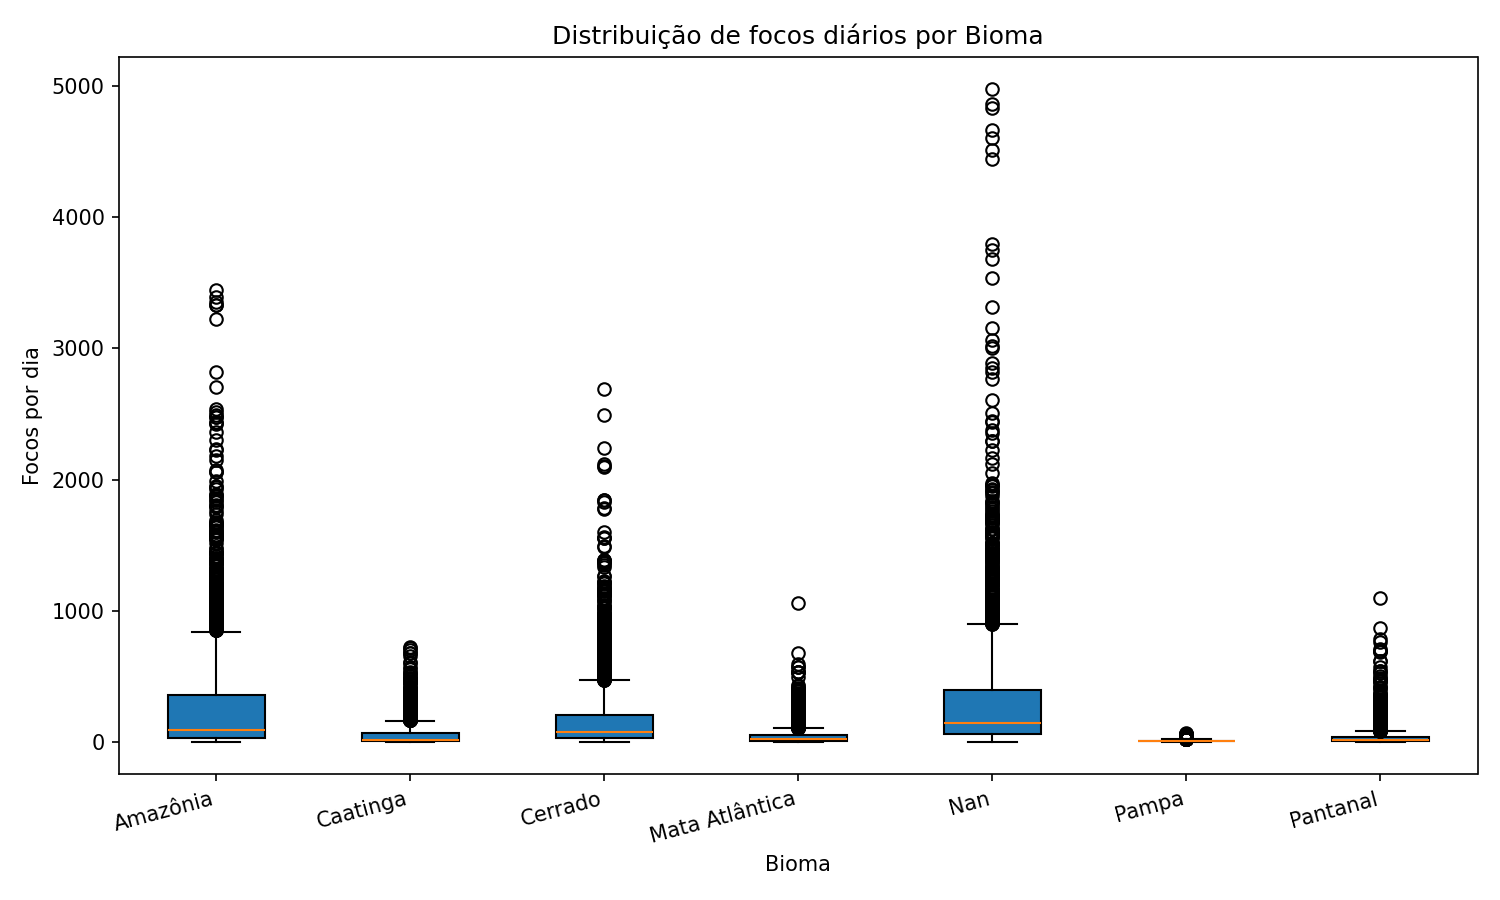
\includegraphics[width=0.85\textwidth]{../figs/eda/boxplot_bioma.png}
\caption{Distribuição de focos mensais por Bioma (2019-2024). O gráfico evidencia a variabilidade e concentração de focos nos diferentes biomas brasileiros, com destaque para Amazônia e Cerrado.}
\label{fig:boxplot_bioma}
\end{figure}

\subsection{Análise dos Top 10 Estados}

A concentração espacial dos focos é um fator crítico para priorização de políticas públicas. A figura a seguir apresenta os 10 estados com maior número de focos registrados no período analisado.

\begin{figure}[h]
\centering
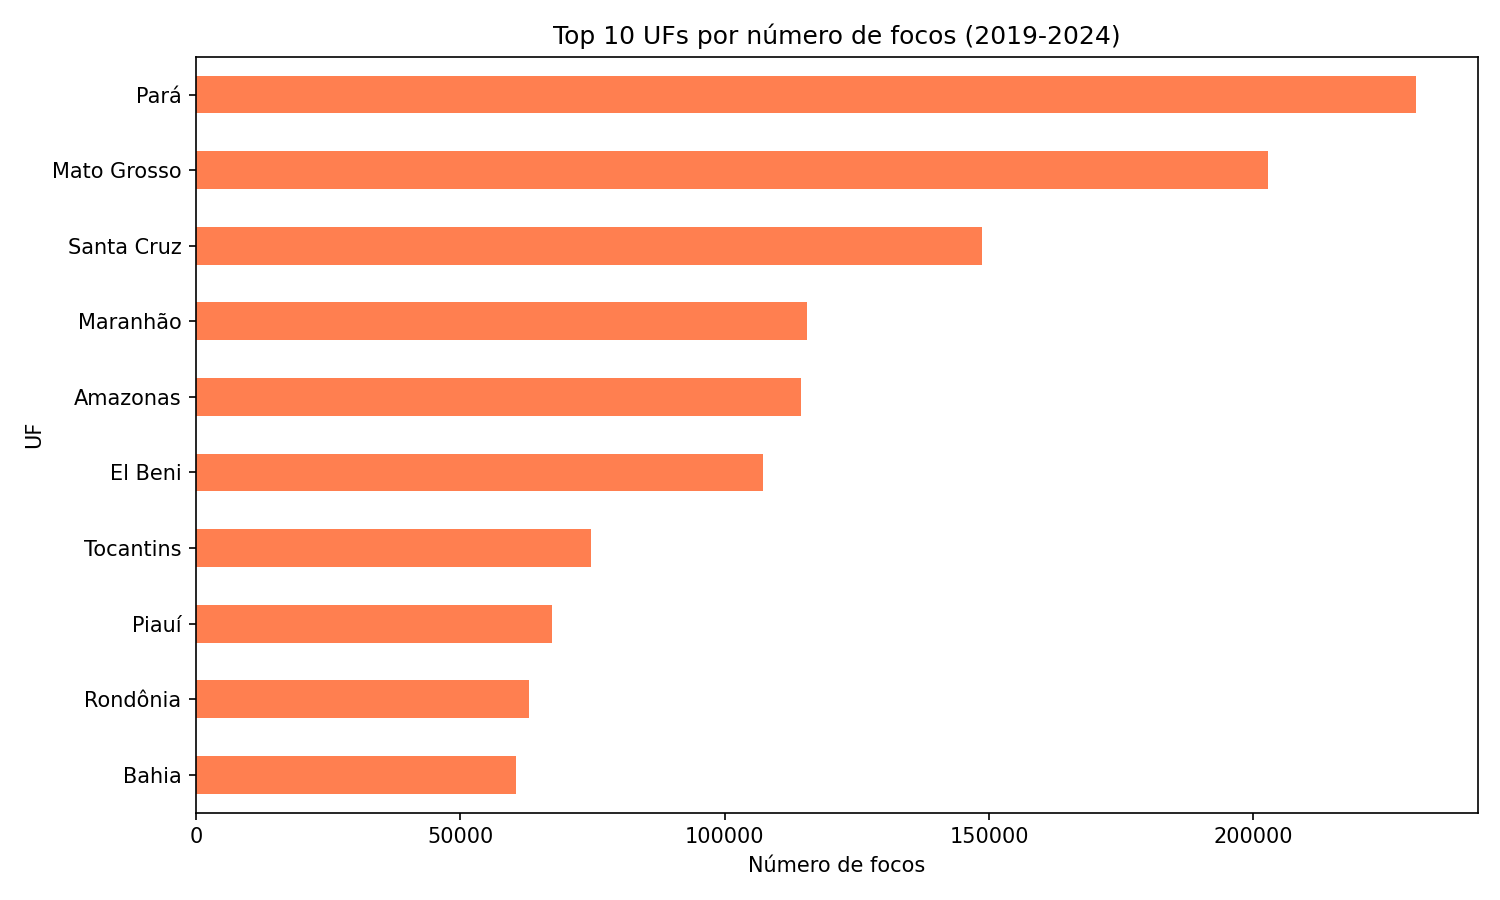
\includegraphics[width=0.85\textwidth]{../figs/eda/top10_uf.png}
\caption{Top 10 UFs por número de focos (2019-2024). Estados da região Norte e Centro-Oeste concentram a maior parte dos focos de queimadas.}
\label{fig:top10_uf}
\end{figure}

\section{Séries Temporais e Sazonalidade}

A análise temporal dos focos de queimadas revela padrões sazonais consistentes ao longo dos anos. A série temporal por bioma demonstra a dinâmica dos focos ao longo do período 2019-2024, permitindo identificar picos sazonais e tendências de longo prazo.

\begin{figure}[h]
\centering
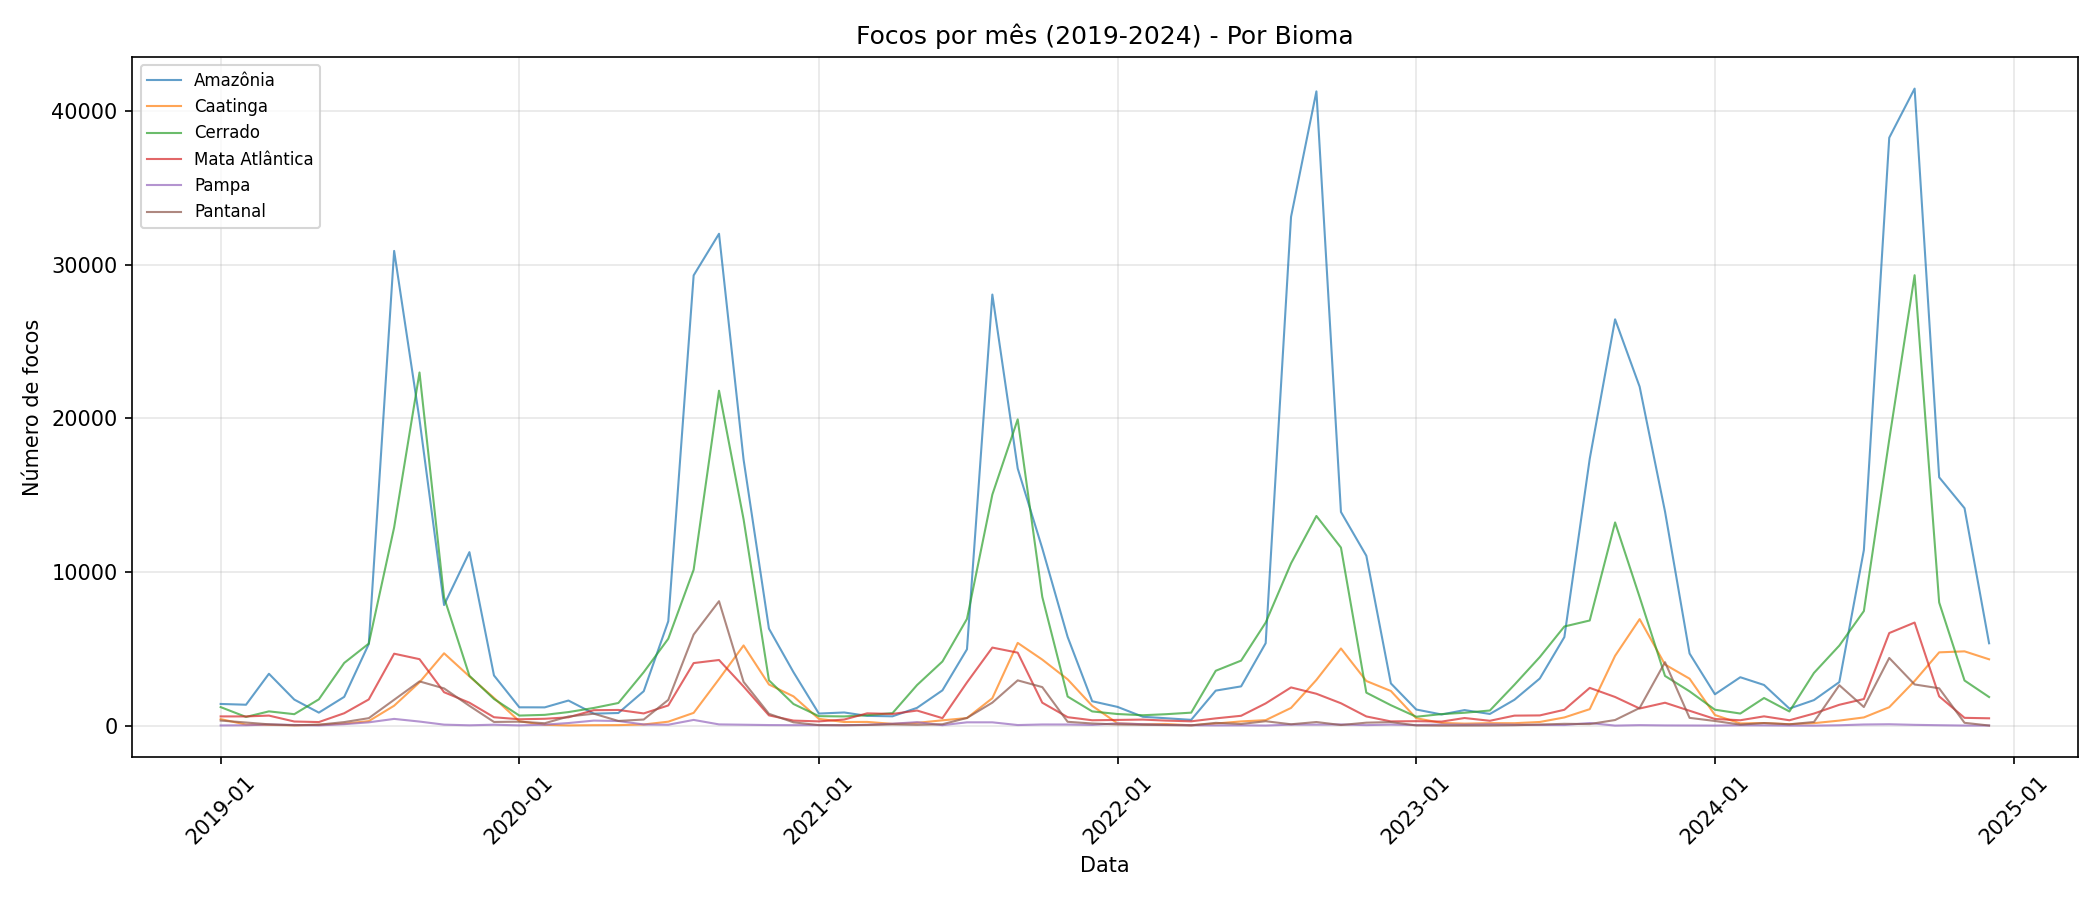
\includegraphics[width=0.95\textwidth]{../figs/eda/series_bioma.png}
\caption{Séries temporais mensais de focos por Bioma (2019-2024). Observa-se clara sazonalidade, com picos concentrados nos meses de seca (julho a outubro), especialmente nos biomas Amazônia e Cerrado.}
\label{fig:series_bioma}
\end{figure}

\subsection{Padrões Observados}

\begin{itemize}
  \item \textbf{Sazonalidade}: Concentração de focos nos meses secos (julho-outubro)
  \item \textbf{Picos históricos}: Anos de 2020 e 2024 apresentam picos significativos
  \item \textbf{Variação por bioma}: Amazônia e Cerrado mostram maior variabilidade
  \item \textbf{Tendência}: Necessário monitoramento contínuo para detecção de mudanças estruturais
\end{itemize}

\section{Outliers e Anomalias}

A detecção de anomalias foi realizada utilizando \textbf{z-score robusto (MAD - Median Absolute Deviation)} sobre as séries temporais diárias. O método identifica dias com número de focos significativamente acima do esperado.

\subsection{Principais Anomalias Detectadas}

Os dias com maior número de focos (anomalias críticas) identificados no período foram:

\begin{table}[h]
\centering
\caption{Top 5 dias com picos anômalos de focos}
\label{tab:anomalias}
\begin{tabular}{lrr}
\toprule
\textbf{Data} & \textbf{Focos} & \textbf{Z-score robusto} \\
\midrule
01/10/2020 & 8.396 & 18.99 \\
07/09/2024 & 8.152 & 18.40 \\
03/09/2024 & 8.073 & 18.22 \\
10/09/2024 & 7.745 & 17.43 \\
05/09/2024 & 7.365 & 16.53 \\
\bottomrule
\end{tabular}
\end{table}

\subsection{Interpretação}

\begin{itemize}
  \item \textbf{Pico histórico}: Outubro de 2020 registrou o maior pico do período
  \item \textbf{Ano recente crítico}: Setembro de 2024 concentra 4 dos 5 maiores picos
  \item \textbf{Padrão temporal}: Anomalias concentram-se no período seco (agosto-outubro)
  \item \textbf{Implicações}: Eventos críticos demandam resposta emergencial coordenada
\end{itemize}

\noindent Lista completa de anomalias disponível em \texttt{data/processed/anomalias\_top.csv}, identificando 50 eventos críticos para análise aprofundada e ações prioritárias.

\section{Síntese da Análise Exploratória}

A análise exploratória de dados realizada sobre mais de 2 milhões de registros de focos de queimadas entre 2019 e 2024 revelou os seguintes achados principais:

\begin{enumerate}
  \item \textbf{Concentração espacial}: Amazônia e Cerrado concentram aproximadamente 50\% dos focos, com estados como Pará, Mato Grosso e Maranhão liderando as ocorrências.
  
  \item \textbf{Padrão sazonal consistente}: Clara concentração de focos nos meses de seca (julho a outubro), com variações anuais significativas que sugerem influência de fatores climáticos e antropogênicos.
  
  \item \textbf{Eventos críticos}: Identificação de picos anômalos, especialmente em outubro/2020 e setembro/2024, que demandam investigação detalhada sobre causas e impactos.
  
  \item \textbf{Qualidade dos dados}: Base consolidada apresenta estrutura adequada para análises preditivas e detecção de anomalias, com tratamento apropriado de valores ausentes e validação de coordenadas geográficas.
  
  \item \textbf{Implicações para modelagem}: Os padrões identificados justificam a proposta analítica de decomposição de séries temporais e detecção de anomalias por métodos estatísticos robustos.
\end{enumerate}

\noindent Os artefatos gerados (figuras, tabelas e CSVs processados) fornecem base sólida para a próxima etapa de modelagem e \textit{data storytelling} orientado à decisão.

% -------------------- Cap. 6: Repositório -----------------------------
\chapter{Repositório e Alinhamento}

\noindent \textbf{Repositório:} \repositorio

\noindent\textbf{Estrutura (alto nível)}: \texttt{data/raw}, \texttt{data/processed}, \texttt{src}, \texttt{notebooks}, \texttt{figs/eda}, \texttt{docs}.  
Scripts e notebook foram desenvolvidos em Python, com comentários, boas práticas e geração automática de artefatos referenciados neste relatório.

% -------------------- Referências -------------------------------------
\chapter*{Referências}
\addcontentsline{toc}{chapter}{Referências}
INPE -- Programa Queimadas (documentação pública).\\
Materiais e orientações do componente curricular.\\
Repositório do projeto: \repositorio

\end{document}
